%\documentclass{beamer} % animation turned ON
\documentclass[handout]{beamer} % animation turned OFF


% PACKAGES
%%%%%%%%%%%%%%%%%%%%%%%%%%%%%%%%%%%%%%%%%%%%%%%%%%%%%%%%%%%%%%%%%%%%%%%%%%%%%%%%

\usepackage{color}
\usepackage{xcolor}
\usepackage{listings}
\usepackage{hyperref}
\usepackage{xifthen}
\usepackage{graphicx}
\graphicspath{ {images/} }
\usepackage{setspace}
\usepackage{ulem} % strike through
\usepackage{textpos}  % textblock


% THEME
%%%%%%%%%%%%%%%%%%%%%%%%%%%%%%%%%%%%%%%%%%%%%%%%%%%%%%%%%%%%%%%%%%%%%%%%%%%%%%%%


\definecolor{kotlinBgDark}{RGB}{20,52,74}
\definecolor{kotlinBgBright}{RGB}{51,109,146}
\definecolor{slidesBgDark}{RGB}{32,39,41}

\definecolor{red}{RGB}{213,32,2}
\definecolor{someBlue}{RGB}{52,138,233}

\newcommand{\textBlue}[1]{\textcolor{someBlue}{#1}}

% https://www.hartwork.org/beamer-theme-matrix/
\mode<presentation>
{
  \usetheme{Rochester}
  \usecolortheme{seagull}
  \setbeamercolor*{frametitle}{fg=white,bg=kotlinBgBright}
}
% get rid of navigation symbols at the bottom
\setbeamertemplate{navigation symbols}{}

\setbeamertemplate{footline}{
    \hfill\scriptsize{\textcolor{kotlinBgBright}{\insertframenumber}}\hspace*{4pt}\vspace{4pt}
}%[frame number]

\hypersetup{
    colorlinks=true,
    linkcolor=kotlinBgBright,
    filecolor=kotlinBgBright,      
    urlcolor=kotlinBgBright,
}

\setbeamertemplate{caption}{\raggedright\footnotesize{\insertcaption}\par}

\addtobeamertemplate{frametitle}{}{
\begin{textblock*}{100mm}(\textwidth,-1cm)

\includegraphics[height=0.6cm]{kotlin_logo_transparent}
\end{textblock*}}


% CUSTOM COMMANDS
%%%%%%%%%%%%%%%%%%%%%%%%%%%%%%%%%%%%%%%%%%%%%%%%%%%%%%%%%%%%%%%%%%%%%%%%%%%%%%%%

\makeatletter
    \newenvironment{withoutheadline}{
        \setbeamertemplate{headline}[default]
        \def\beamer@entrycode{\vspace*{-\headheight}}
    }{}
\makeatother

\newcommand{\quotes}[1]{
  \linespread{1.3}\selectfont
  ``\large{\textit{#1}}''\par\bigskip
  \linespread{1}\selectfont % reset
}

\newcommand{\fullimage}[1]{
\begin{withoutheadline}
\frame{
\begin{figure}[h]
  \centering
  \includegraphics[width=10cm]{#1}
\end{figure}
}
\end{withoutheadline}
}


\newenvironment{whiteframe}
{
\begin{withoutheadline}
\begin{frame}
%\begin{figure}[h]
%\begin{center}
\center
}
{
%\end{center}
%\end{figure}
\end{frame}
\end{withoutheadline}
}

\newcommand{\fulltitle}[1]{
\begin{whiteframe}
\Huge{#1}
\end{whiteframe}
}


\newcommand{\fullimageCapt}[3]{
\begin{withoutheadline}
\frame{
\begin{figure}[h]
  \centering
  \ifthenelse{\equal{#3}{}}{\includegraphics[width=10cm]{#1}}{\includegraphics[width=#3]{#1}}
%\includegraphics[width=10cm]{#1}
  \caption{#2}
\end{figure}
}
\end{withoutheadline}
}

\newcommand\sektion[1]{
  \section{#1}
% http://tex.stackexchange.com/questions/44983/beamer-removing-headline-and-its-space-on-a-single-frame-for-plan-but-keepin
{
\setbeamertemplate{footline}{}
\setbeamercolor{frametitle}{bg=slidesBgDark} {
\setbeamercolor{background canvas}{bg=slidesBgDark} {
  \frame{
    \textbf{\huge\textcolor{white}{#1}}
    \noindent\makebox[\linewidth]{\textcolor{kotlinBgBright}{\rule{\paperwidth}{1.4pt}}} % http://tex.stackexchange.com/questions/88502/how-to-change-the-shaded-color-of-the-rule-command
  }}
}
}
}

% LISTING
%%%%%%%%%%%%%%%%%%%%%%%%%%%%%%%%%%%%%%%%%%%%%%%%%%%%%%%%%%%%%%%%%%%%%%%%%%%%%%%%

\definecolor{IJ_text}{RGB}{169,183,198}
\definecolor{IJ_background}{RGB}{43,43,43}
\definecolor{IJ_keyword}{RGB}{204,120,50}
\definecolor{IJ_string}{RGB}{106,135,89}
\definecolor{IJ_comment}{RGB}{128,128,128}
\definecolor{IJ_identifier}{RGB}{255,198,109}

% https://en.wikibooks.org/wiki/LaTeX/Source_Code_Listings
% http://tex.stackexchange.com/questions/28229/extend-a-language-with-additional-keywords
\lstset{language=Java}
\lstset{
 morekeywords={if, else, fun, val, var, get, set, data, enum, when, inline, object, infix, override, is, lateinit, companion, init}
}
\lstset{
    backgroundcolor=\color{IJ_background},
    basicstyle=\color{IJ_text}\ttfamily,
%    basicstyle=\small\ttfamily,%
% NOPE    breaklines=true,
    captionpos=b, % sets the caption-position to bottom
    commentstyle=\color{IJ_comment}\ttfamily,
%    columns=fullflexible,
    escapeinside=||,
    framexleftmargin=4pt,
%    framerule=0pt,
    frame=none,
    keywordstyle=\color{IJ_keyword}\ttfamily,
    stepnumber=1,
    numbersep=6pt,
    numbers=left, % numbers=none,
    numberstyle=\tiny,
    stringstyle=\color{IJ_string}\ttfamily,
% NO! as java vs kotlin issue :( identifierstyle=\color{IJ_identifier}\ttfamily,
    showstringspaces=false
}%
%\lstset{framesep=10pt}
%\lstset{xleftmargin=10pt,xrightmargin=10pt}
%\lstset{emph={%  
%    val, var%
%    },emphstyle={\color{red}\bfseries\underbar}%
%}%


\lstdefinestyle{twosided}
{
  basicstyle=\color{IJ_text}\ttfamily\tiny, %or \small or \footnotesize etc.
  numbers=none,
  framexleftmargin=2pt
}


% MISC
%%%%%%%%%%%%%%%%%%%%%%%%%%%%%%%%%%%%%%%%%%%%%%%%%%%%%%%%%%%%%%%%%%%%%%%%%%%%%%%%



\begin{document}

\title{Kotlin meets Gadsu}   
\author{Christoph Pickl} 
\date{\today} 

\section{Kotlin meets Gadsu}
{
\setbeamertemplate{footline}{}
\setbeamercolor{frametitle}{bg=slidesBgDark} {
\setbeamercolor{background canvas}{bg=slidesBgDark} {
  \frame{
    
\includegraphics[height=0.6cm]{kotlin_logo_transparent}\textbf{\Huge\textcolor{white}{otlin meets Gadsu}}

    \noindent\makebox[\linewidth]{\textcolor{kotlinBgBright}{\rule{\paperwidth}{1.4pt}}}
    \vspace{2.0pt} \\
    \textbf{\large{\textcolor{white}{Christoph Pickl}}} \\
    \textbf{\scriptsize{\textcolor{white}{Kotlin Vienna Meetup -- 2017-01-31}}}
  }
}
}
}


\frame{\frametitle{Agenda} 

\setbeamercolor{normal text}{fg=gray,bg=}
\setbeamercolor{alerted text}{fg=black,bg=}
\usebeamercolor{normal text}

\begin{enumerate}
	\item \alert<+>{Introduction to Gadsu} % the app and a bit theory behind shiatsu, TCM; future features of gadsu
	\item \alert<+>{Kotlin in the wild} % tooling & infrastructure: gradle, travis, version eye, coverage
	\item \alert<+>{Code ``\textit{Schmankerln}''} % most practical code snippets/language features; frameworks&libs
	\item \alert<+>{Lessons Learned} % summarize highlights
\end{enumerate}
}

\sektion{Introduction to Gadsu}

%%%%%%%%%%%%%%%%%%%%%%%%%%%%%%%%%%%%%%%%%%%%%%%%
\fullimageCapt{gadse}{This is a cat.}{8cm}

%%%%%%%%%%%%%%%%%%%%%%%%%%%%%%%%%%%%%%%%%%%%%%%%
\fullimageCapt{ohashi}{This is Shiatsu.}{6.3cm}

%%%%%%%%%%%%%%%%%%%%%%%%%%%%%%%%%%%%%%%%%%%%%%%%
\frame{\frametitle{Gadsu is \ldots} 
\pause
\begin{center}
\begin{Huge}
Gadse
\pause

\vspace{0.5cm}

+ Shiatsu
\pause

\vspace{0.8cm}

= Gadsu
\end{Huge}
\end{center}

}
%%%%%%%%%%%%%%%%%%%%%%%%%%%%%%%%%%%%%%%%%%%%%%%%
\fullimageCapt{gadsu_screenshot}{Visit \href{https://github.com/christophpickl/gadsu}{github.com}}{11cm}

%%%%%%%%%%%%%%%%%%%%%%%%%%%%%%%%%%%%%%%%%%%%%%%%
\frame{\frametitle{Shiatsu is \ldots}

\begin{itemize}
	\item Acpuressure, meridian therapy, physio therapy, massage, stimulation of the nervous system, life coaching
	\item Based on the \textbf{T}raditional \textbf{C}hinese \textbf{M}edicine
	\begin{itemize}
		\item Body and mind seen as a unit, not separated from each other
		\item Concepts like Qi, 5 Elements
	\end{itemize}
\end{itemize}

\begin{figure}[h]
\centering
  
\includegraphics[height=2.0cm]{yinyang}
\end{figure}
}

%%%%%%%%%%%%%%%%%%%%%%%%%%%%%%%%%%%%%%%%%%%%%%%%
\begin{frame}[t]
\frametitle{Features}
\begin{columns}[t]
\begin{column}{0.5\textwidth}
	Present:
	\begin{itemize}
		\item Manage clients, appointments, diagnosis and treatments
		\item Manage medical record
		\item Reporting
		\item GMail integration
		\item Google Calendar integration
		\item Native executables
		\item Auto update software
		\item Auto backup data
	\end{itemize}
\end{column}
\begin{column}{0.5\textwidth} 
	Future:
	\begin{itemize}
		\item TCM assistant
		\item Statistics
		\item Pain indicator
		\item 5 Element widget
		\item Invoicing
		\item Doodle integration
		\item Search / sort clients
	\end{itemize}
\end{column}
\end{columns}
\end{frame}

%%%%%%%%%%%%%%%%%%%%%%%%%%%%%%%%%%%%%%%%%%%%%%%%
\begin{frame}
\frametitle{Technology Stack}
\begin{itemize}
	\item Gradle
	\item Swing
	\item Guice
	\item Spring JDBC
	\item HSQLDB + Flyway
	\item Jasper, Pdfbox
	\item Freemarker
	\item TestNG, Mockito, Hamcrest
	\item UISpec4J
\end{itemize}

\end{frame}


\sektion{
\includegraphics[height=0.6cm]{kotlin_logo_transparent}otlin in the wild}


%%%%%%%%%%%%%%%%%%%%%%%%%%%%%%%%%%%%%%%%%%%%%%%%
\begin{frame}[fragile] \frametitle{\texttt{build.gradle}}
\begin{lstlisting}
apply plugin: "kotlin"|\pause|
buildscript {
  ext.kotlin_version = '1.0.6'
  dependencies {
    classpath "org.jetbrains.kotlin:
      kotlin-gradle-plugin:$kotlin_version"
  }
}|\pause|
dependencies {
  compile "org.jetbrains.kotlin:
    kotlin-stdlib:$kotlin_version"
  compile "org.jetbrains.kotlin:
    kotlin-reflect:$kotlin_version"
}
\end{lstlisting}
\end{frame}

%%%%%%%%%%%%%%%%%%%%%%%%%%%%%%%%%%%%%%%%%%%%%%%%
\fullimageCapt{travis}{\href{https://travis-ci.org/christophpickl/gadsu}{travis-ci.org}}{10cm}

\begin{frame}[fragile] \frametitle{\texttt{.travis.yml}}
\begin{lstlisting}
language: kotlin|\pause|
sudo: false|\pause|
jdk:
  - oraclejdk8|\pause|
before_install:
  - "chmod +x gradlew"|\pause|
  - "export DISPLAY=:99.0"
  - "sh -e /etc/init.d/xvfb start"|\pause|
script:
  - "./gradlew test ..."|\pause|
notifications:
  email:
    - "MLtravis@gadsu.com"
\end{lstlisting}
\end{frame}

%%%%%%%%%%%%%%%%%%%%%%%%%%%%%%%%%%%%%%%%%%%%%%%%
\fullimageCapt{codecov}{\href{https://codecov.io/gh/christophpickl/gadsu/}{codecov.io}}{10cm}

\begin{frame}[fragile] \frametitle{Codecov} 
Gradle Configuration:

\begin{lstlisting}
plugins {
  id 'jacoco'
  id 'com.github.kt3k.coveralls'
}|\pause|
jacocoTestReport {
  reports {
    xml.enabled = true
}}
\end{lstlisting}
\pause

Travis Configuration:

\begin{lstlisting}
script:
  - "./gradlew ... jacocoTestReport ..."|\pause|
after_success:
  - bash <(curl -s https://codecov.io/bash)
\end{lstlisting}


\end{frame}


%%%%%%%%%%%%%%%%%%%%%%%%%%%%%%%%%%%%%%%%%%%%%%%%
\fullimageCapt{versioneye}{\href{https://www.versioneye.com/user/projects/572880644a0faa000b782062}{versioneye.com}}{10cm}

\begin{frame}[fragile] \frametitle{VersionEye} 
Gradle Configuration:
\begin{lstlisting}
plugins {
  id "org.standardout.versioneye"
    version "1.4.0"
}
\end{lstlisting}
\pause

Gradle Properties:
\begin{lstlisting}
versioneye.projectid=572880644a0f...00b78206
\end{lstlisting}
\pause


Travis Configuration:

\begin{lstlisting}
script:
  - "./gradlew ... versioneye-update ..."
\end{lstlisting}
 
\end{frame}


\begin{frame} \frametitle{VersionEye GitHub Integration} 

\centering{Display coverage data via the \href{https://github.com/codecov/browser-extension}{Codecov Browser Extension}:}

\begin{figure}[h]
\centering
  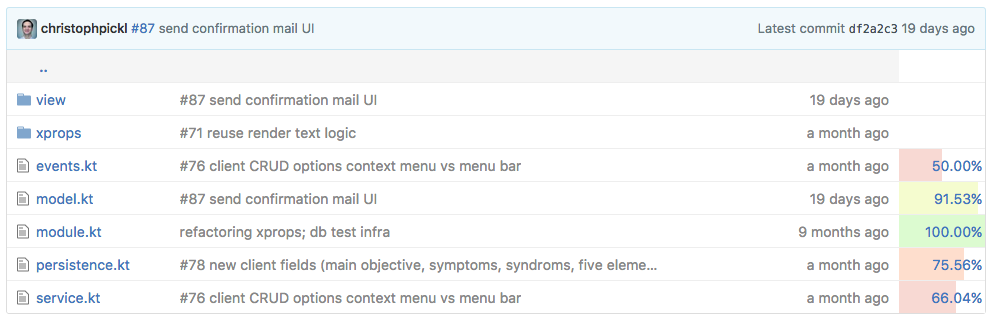
\includegraphics[width=10cm]{versioneye_github1}
\end{figure}
\begin{figure}[h]
\centering
  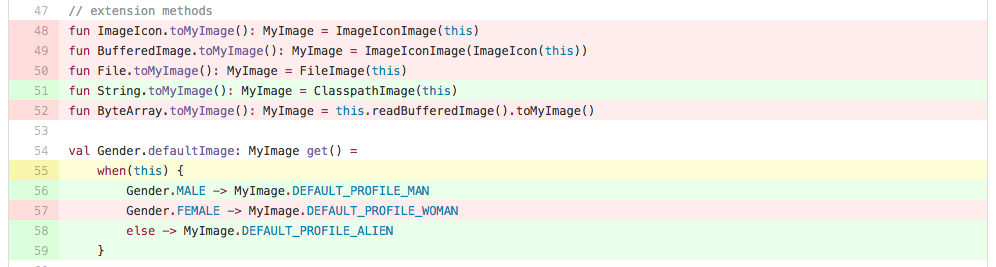
\includegraphics[width=10cm]{versioneye_github2}
\end{figure}
\end{frame}


\sektion{Code Schmankerln}


%%%%%%%%%%%%%%%%%%%%%%%%%%%%%%%%%%%%%%%%%%%%%%%%
\begin{frame}[fragile] \frametitle{Extension Methods \#1}
The \textit{neutral} \textbf{domain object}:
\begin{lstlisting}
package at.cpickl.gadsu.client

data class Client(
  val id: String,
  val name: String
)
\end{lstlisting}
\end{frame}

%%%%%%%%%%%%%%%%%%%%%%%%%%%%%%%%%%%%%%%%%%%%%%%%
\begin{frame}[fragile] \frametitle{Extension Methods \#2}
\textbf{Persistence} specific functionality:
\begin{lstlisting}
package at.cpickl.gadsu.persistence

data class ClientDbo(
  val TXT_ID: String,
  val TXT_NAME: String
)|\pause|
fun Client.toDbo() =
        ClientDbo(id, name)
|\pause|
class ClientRepo {
    fun save(client: Client) {
        saveSomewhere(client.toDbo())
    }
}
\end{lstlisting}
\end{frame}


%%%%%%%%%%%%%%%%%%%%%%%%%%%%%%%%%%%%%%%%%%%%%%%%
\begin{frame}[fragile] \frametitle{Extension Methods \#3}
Add a \textbf{fluent API} to an existing classes:
\begin{lstlisting}
fun <T : JComponent> T.bold(): T {
  font = font.deriveFont(Font.BOLD)
  return this
}
|\pause|
val myLabel = JLabel("text").bold()
val myTextField = JTextField("text").bold()
val myTextArea = JTextArea("text").bold()
\end{lstlisting}
\end{frame}

%%%%%%%%%%%%%%%%%%%%%%%%%%%%%%%%%%%%%%%%%%%%%%%%
\begin{frame}[fragile] \frametitle{Extension Properties \#1}
Possible replacement of common \textbf{test factories}:
\begin{lstlisting}
package at.cpickl.gadsu.test

val Client.Companion.testee1: Client
  get() = Client(
    id = "",
    name = "Max Muster"
)
\end{lstlisting}
\pause

Sadly requires to have some \textit{placeholder}:
\begin{lstlisting}
package at.cpickl.gadsu.client

data class Client( ... ) {
    companion object {}
}
\end{lstlisting}
\end{frame}

%%%%%%%%%%%%%%%%%%%%%%%%%%%%%%%%%%%%%%%%%%%%%%%%
\begin{frame}[fragile] \frametitle{Extension Properties \#2}
Use those testees in your \textbf{tests}:
\begin{lstlisting}
package at.cpickl.gadsu.test

@Test class ClientIT {

  @Inject lateinit var repo: ClientRepo
  
  fun `reference test scoped testee`() {
    repo.save(
      Client.testee1.copy(name = "Otto")
    )
    // ... assertions ... 
  }
}
\end{lstlisting}
\end{frame}


%%%%%%%%%%%%%%%%%%%%%%%%%%%%%%%%%%%%%%%%%%%%%%%%
\begin{frame}[fragile] \frametitle{Function done right}

TODO TODO TODO TODO TODO TODO TODO 

Java 8
\begin{lstlisting}
Collection, filter, map, STREAM!, collector
\end{lstlisting}

Kotlin (implicit \texttt{it} variable)
\begin{lstlisting}
Collection, filter, map
\end{lstlisting}
\end{frame}


%%%%%%%%%%%%%%%%%%%%%%%%%%%%%%%%%%%%%%%%%%%%%%%%
\fullimageCapt{lazy}{Sometimes I feel so lazy \ldots}{8cm}

%%%%%%%%%%%%%%%%%%%%%%%%%%%%%%%%%%%%%%%%%%%%%%%%
\begin{frame}[fragile] \frametitle{Lazy in Java}
Given there is a \textit{very expensive} \texttt{expensiveInit()} method:
\pause
\begin{lstlisting}
public class NaiveSingleton {
  private Object lazyField = null;

  public Object getLazyField() {
    if (lazyField == null) {
      lazyField = expensiveInit();
    }
    return lazyField;
  }
}
\end{lstlisting}
\end{frame}

%%%%%%%%%%%%%%%%%%%%%%%%%%%%%%%%%%%%%%%%%%%%%%%%
\begin{frame}[fragile] \frametitle{Lazy in Java8}
\begin{lstlisting}
public class Java8 {
  private Supplier<Object> lazyField=() -> {
    Object value = expensiveInit();
    lazyField = () -> value;
    return value;
  };

  public Object getLazyField() {
    return lazyField.get();
  }
}
\end{lstlisting}
\end{frame}

%%%%%%%%%%%%%%%%%%%%%%%%%%%%%%%%%%%%%%%%%%%%%%%%
\begin{frame}[fragile] \frametitle{Lazy in Kotlin}
\begin{lstlisting}
class LazyKotlin {
  val lazyField by lazy {
    expensiveInit()
  }
}|\pause|

// part of stdlib:
fun <T> lazy(initializer: ()->T): Lazy<T> =
  SynchronizedLazyImpl(initializer)
\end{lstlisting}
\pause
Thanks to type inference, we don't need to specify types explicity.
\end{frame}


%%%%%%%%%%%%%%%%%%%%%%%%%%%%%%%%%%%%%%%%%%%%%%%%
\begin{frame}[fragile] \frametitle{Class Delegation}
Given the existing classes:
\begin{lstlisting}
interface Step {
  fun take()
}|\pause|

class StepImpl : Step {
  override fun take() {}
}
\end{lstlisting}
\pause
We now want some new service to implement this interface, \\
but \textbf{delegate} all its methods to the \texttt{StepImpl} implementation.
\end{frame}

\begin{frame}[fragile] \frametitle{Reimplement in Java}
\begin{lstlisting}
public class MyService implements Step {

  private final Step step;
  
  public MyService(Step step) {
    this.step = step;
  }
  
  @Override public void take() {
    step.take();
  }
}
\end{lstlisting}
\end{frame}


\begin{frame}[fragile] \frametitle{Delegate by Kotlin}
\begin{lstlisting}
class MyService(step: Step) : Step by step
\end{lstlisting}
\pause
\vspace{0.5cm}
Standard delegates in Kotlin:
\begin{itemize}
	\item lazy
	\item observable
	\item map properties
\end{itemize}
\end{frame}



\sektion{Lessons Learned}


%%%%%%%%%%%%%%%%%%%%%%%%%%%%%%%%%%%%%%%%%%%%%%%%
\begin{frame}
\frametitle{Kotlin is a great language}
\begin{itemize}
	\item Null handling is a MUST!
	\item Extension methods for better auto completion
	\item Named and default arguments, data classes
	\item Requires developers to be more disciplined
	\begin{itemize}
		\item Several classes in one (big) file gets common
		\item Overuse of single-expression functions
		\item Overuse of \texttt{apply\{\}}
		\item Explicit type declaration for documentation
	\end{itemize}
\end{itemize}
\end{frame}


%%%%%%%%%%%%%%%%%%%%%%%%%%%%%%%%%%%%%%%%%%%%%%%%
\begin{frame}
\frametitle{Tooling infrastructure grows}
\begin{itemize}
	\item Mostly same as for Java
	\item Build system support (gradle with kotlin coming!)
	\item Static code analysis tools missing
	\item Syntax highlighting mostly missing
\end{itemize}
\end{frame}

%* the "1-liner challenge": no references, just a = method
%* overdoing it with apply (who is this?)
%* data classes are restricted in usage => kotlin 1.1



\end{document}
